\section{Por que uma nuvem?}

Ao consultar livros de redes, telecomunicações e afins, é provável que sempre
encontremos desenhos de nuvens usados para fins de abstração. Nesse sentido, a
ilustração representa uma rede de algum tipo cuja estrutura não precisa ser
conhecida, pelo menos não naquele momento.

Se a intenção em determinado capítulo é explicar como funciona uma tecnologia de
comunicação que interliga duas redes de computadores, por exemplo, não é
necessário detalhar as características de cada uma delas. Assim, o autor pode
utilizar uma nuvem --- a abstração --- para indicar que há redes ali.

A computação em nuvem simplesmente absorveu essa ideia, até porque o desenho de
uma nuvem, no mesmo contexto de abstração, passou também a representar a
internet.

\begin{figure}[ht]
    \centering
    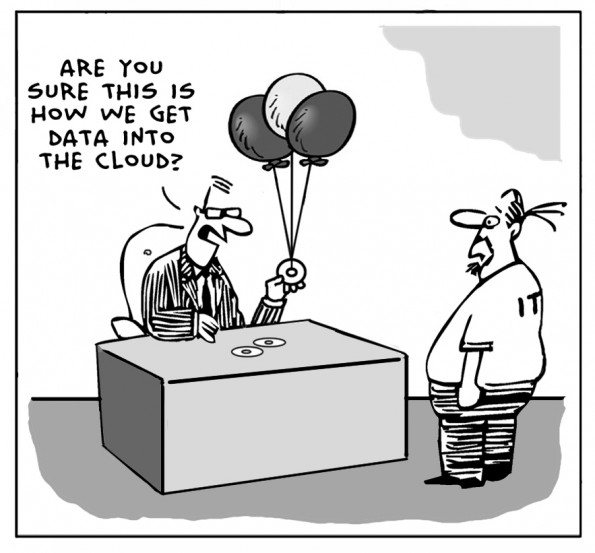
\includegraphics[height=0.3\textwidth]{img/comic.jpg}
    \caption{Charge retratando a "entrada de dados" na nuvem}
\end{figure}
